\documentclass[border=8pt]{standalone}
\usepackage{tikz}

\definecolor{wallcream}{RGB}{245,232,210}
\definecolor{floorwood}{RGB}{166,118,72}
\definecolor{floorlight}{RGB}{188,140,92}
\definecolor{curtainrose}{RGB}{196,110,118}
\definecolor{curtaindark}{RGB}{148,72,82}
\definecolor{sofabeige}{RGB}{186,150,118}
\definecolor{sofacush}{RGB}{210,176,142}
\definecolor{tvframe}{RGB}{52,54,58}
\definecolor{tvscreen}{RGB}{72,118,168}
\definecolor{tvglow}{RGB}{140,178,220}
\definecolor{tableoak}{RGB}{140,96,58}
\definecolor{lampshade}{RGB}{240,210,150}
\definecolor{lampglow}{RGB}{255,230,170}
\definecolor{skin}{RGB}{232,196,168}
\definecolor{hairgray}{RGB}{180,178,176}
\definecolor{dress}{RGB}{120,148,132}
\definecolor{slippers}{RGB}{120,90,70}
\definecolor{rugwarm}{RGB}{198,140,100}
\definecolor{pictureframe}{RGB}{130,95,60}
\definecolor{plantleaf}{RGB}{90,140,95}
\definecolor{pot}{RGB}{170,110,85}

\begin{document}
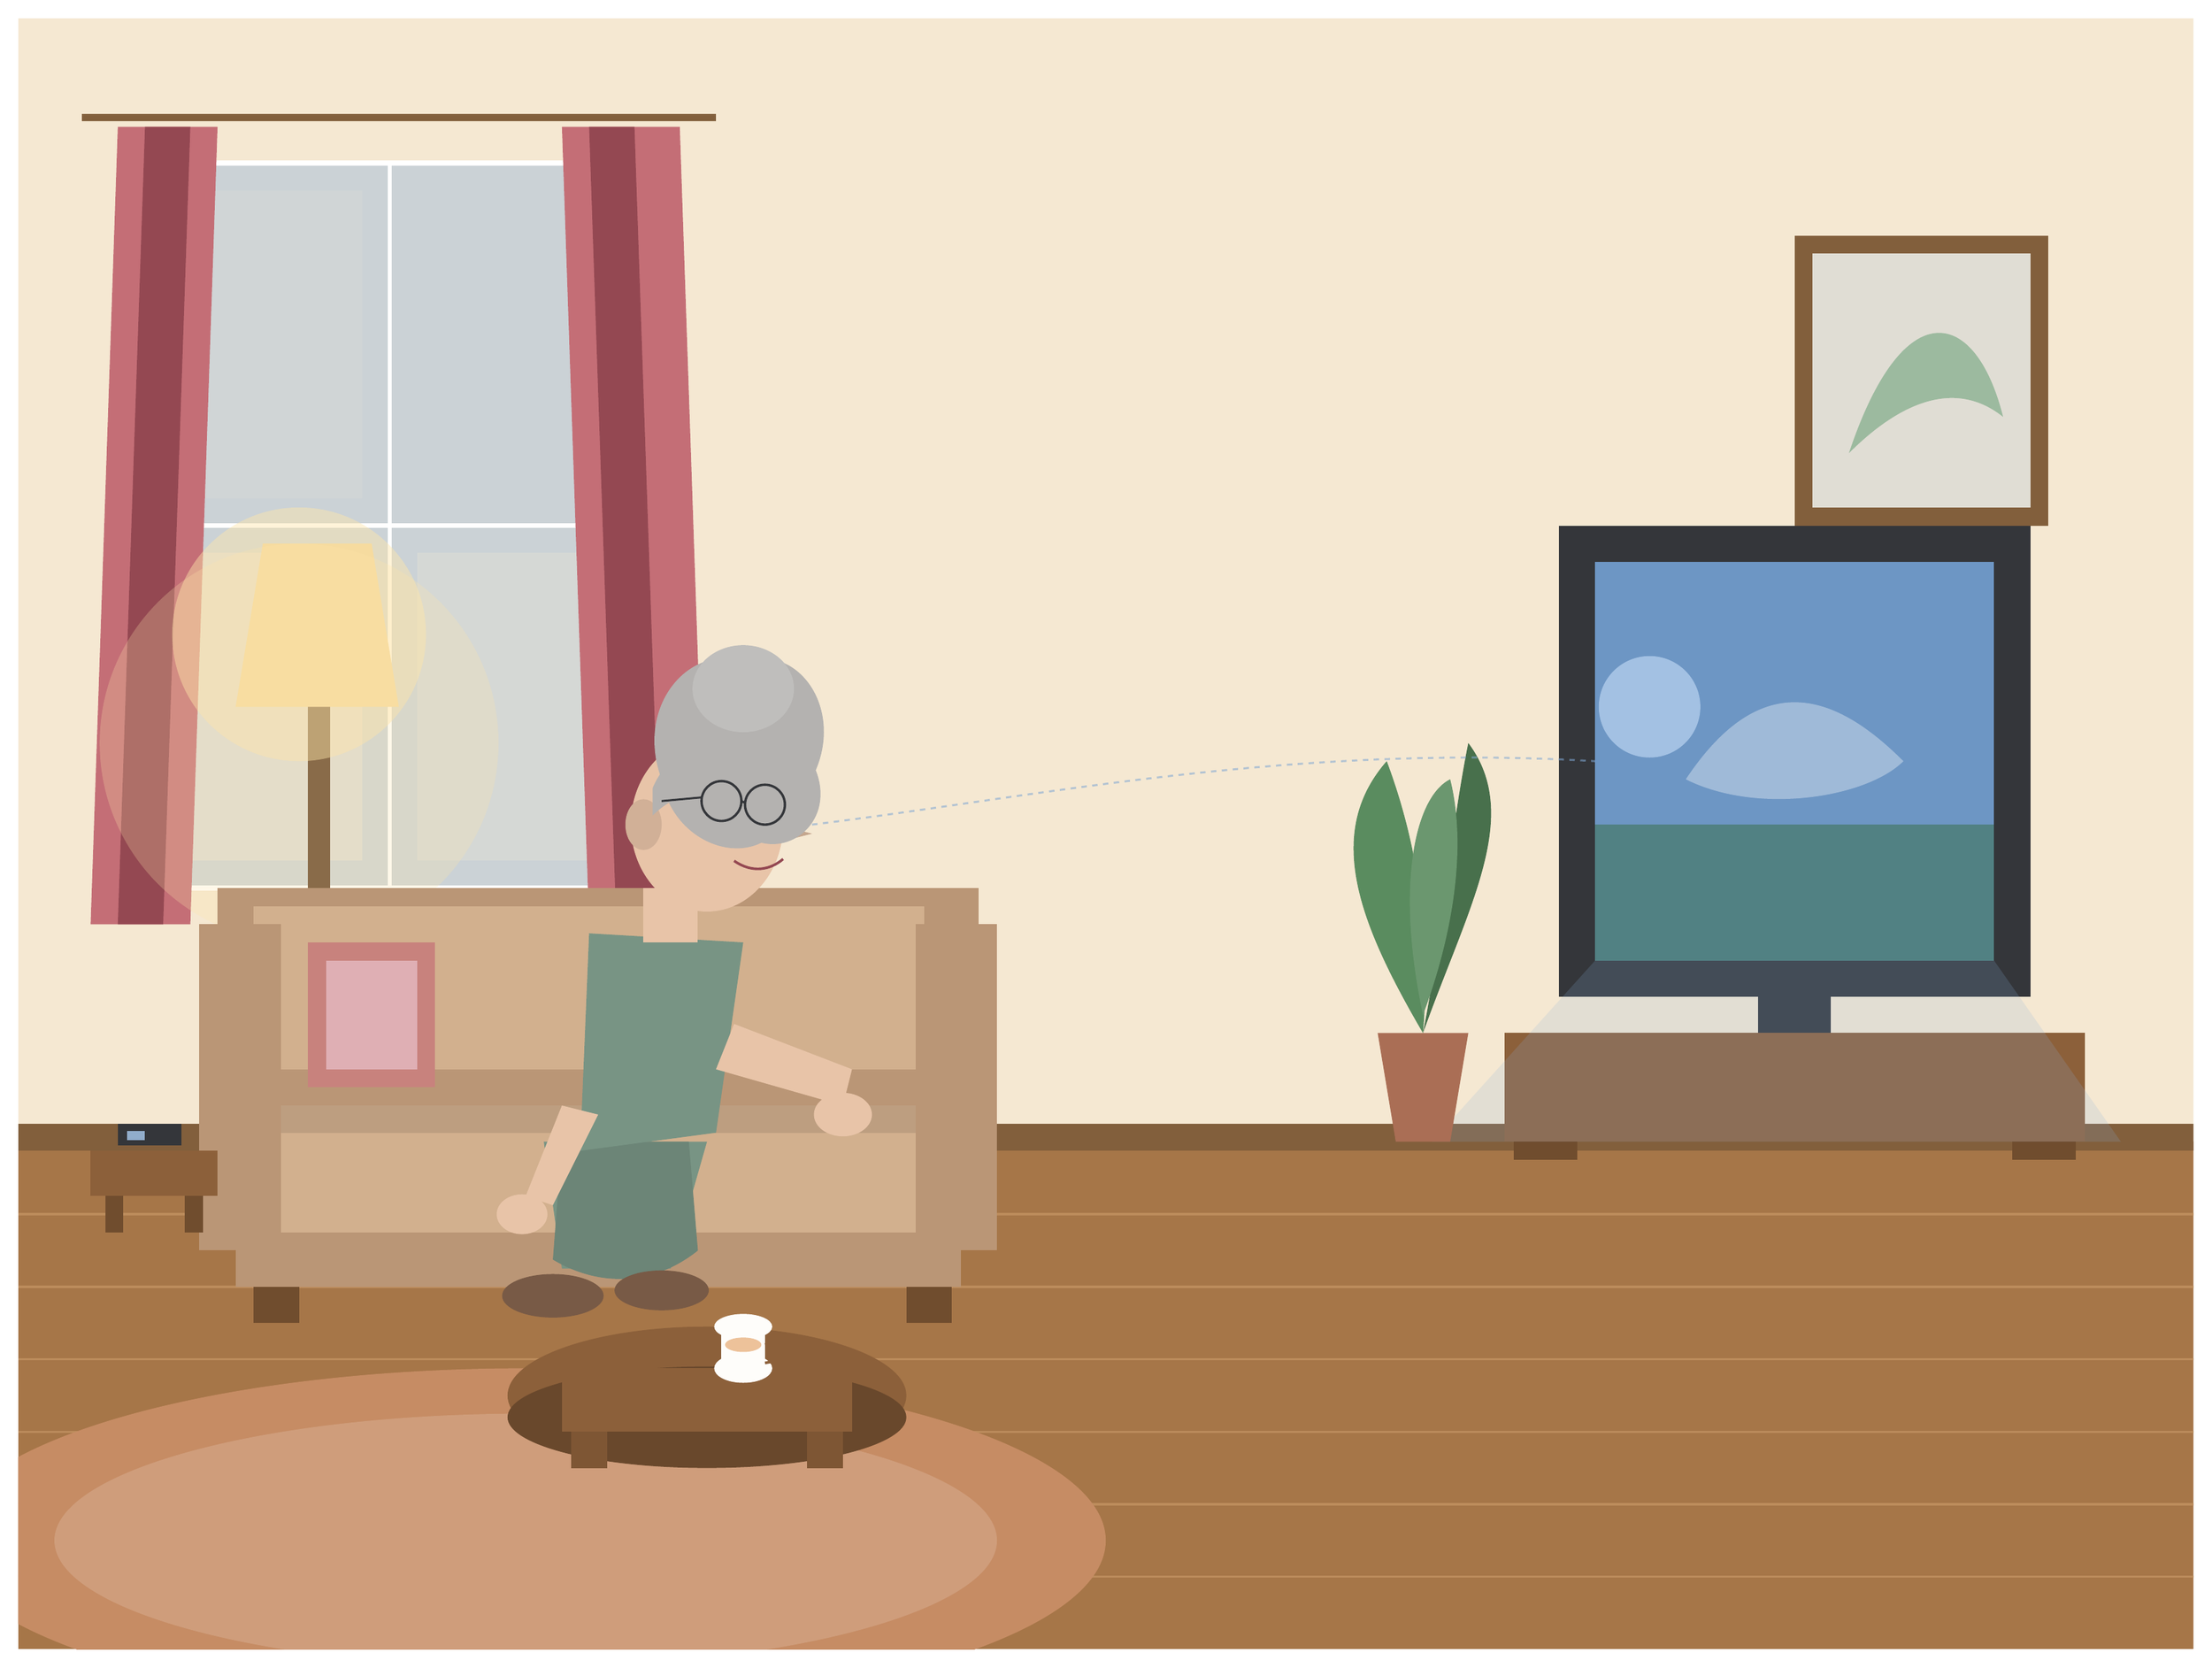
\begin{tikzpicture}[x=1pt,y=1pt]
  % canvas ~1200x900
  \clip (0,0) rectangle (1200,900);

  % --- walls & floor ---
  \fill[wallcream] (0,280) rectangle (1200,900);
  \fill[floorwood] (0,0) rectangle (1200,280);
  % floor boards
  \foreach \y in {40,80,120,160,200,240} {
    \draw[floorlight,line width=1.2pt] (0,\y) -- (1200,\y);
  }
  % baseboard
  \fill[pictureframe] (0,275) rectangle (1200,290);

  % --- window + curtains (left back) ---
  \fill[tvglow!40!wallcream] (70,420) rectangle (340,820);
  % window panes
  \draw[white,line width=3pt] (70,420) rectangle (340,820);
  \draw[white,line width=2.5pt] (205,420) -- (205,820);
  \draw[white,line width=2.5pt] (70,620) -- (340,620);
  % soft outdoor hint
  \fill[tvglow!25!wallcream] (85,435) rectangle (190,605);
  \fill[tvglow!30!wallcream] (220,435) rectangle (325,605);
  \fill[tvglow!35!wallcream] (85,635) rectangle (190,805);
  \fill[tvglow!40!wallcream] (220,635) rectangle (325,805);
  % curtains
  \fill[curtainrose] (40,400) -- (95,400) -- (110,840) -- (55,840) -- cycle;
  \fill[curtaindark] (55,400) -- (80,400) -- (95,840) -- (70,840) -- cycle;
  \fill[curtainrose] (315,400) -- (380,400) -- (365,840) -- (300,840) -- cycle;
  \fill[curtaindark] (330,400) -- (355,400) -- (340,840) -- (315,840) -- cycle;
  % curtain rod
  \draw[pictureframe,line width=4pt] (35,845) -- (385,845);

  % --- wall picture ---
  \fill[pictureframe] (980,620) rectangle (1120,780);
  \fill[wallcream!80!tvglow] (990,630) rectangle (1110,770);
  \fill[plantleaf!60] (1010,660) .. controls (1040,750) and (1080,740) .. (1095,680)
    .. controls (1070,700) and (1040,690) .. (1010,660);

  % --- TV stand + TV (right side) ---
  \fill[tableoak] (820,280) rectangle (1140,340);
  \fill[tableoak!80!black] (825,270) rectangle (860,280);
  \fill[tableoak!80!black] (1100,270) rectangle (1135,280);
  % TV body
  \fill[tvframe] (850,360) rectangle (1110,620);
  % screen with soft glow content
  \fill[tvscreen] (870,380) rectangle (1090,600);
  \fill[tvglow,opacity=0.55] (870,380) rectangle (1090,600);
  % simple on-screen scene (landscape show)
  \fill[plantleaf!50!tvscreen] (870,380) rectangle (1090,455);
  \fill[tvglow!80!white] (900,520) circle (28);
  \fill[white,opacity=0.35] (920,480) .. controls (960,540) and (1000,530) .. (1040,490)
    .. controls (1020,470) and (960,460) .. (920,480);
  % TV stand feet
  \fill[tvframe] (960,340) rectangle (1000,360);
  % screen glow on floor / air
  \fill[tvglow,opacity=0.18] (780,280) -- (870,380) -- (1090,380) -- (1160,280) -- cycle;

  % --- rug ---
  \fill[rugwarm] (280,60) ellipse (320 and 95);
  \fill[rugwarm!85!white] (280,60) ellipse (260 and 70);

  % --- coffee table ---
  \fill[tableoak] (380,140) ellipse (110 and 38);
  \fill[tableoak!75!black] (380,128) ellipse (110 and 28);
  \fill[tableoak] (300,120) rectangle (460,155);
  \fill[tableoak!90!black] (305,100) rectangle (325,120);
  \fill[tableoak!90!black] (435,100) rectangle (455,120);
  % teacup on table
  \fill[white!90!wallcream] (400,155) ellipse (16 and 8);
  \fill[white!90!wallcream] (388,155) rectangle (412,178);
  \fill[white!90!wallcream] (400,178) ellipse (16 and 7);
  \draw[tableoak,line width=1.5pt] (412,168) .. controls (428,172) and (428,160) .. (412,158);
  \fill[lampglow!70!curtainrose] (400,168) ellipse (10 and 4);

  % --- floor lamp (behind sofa left) ---
  \fill[tableoak!70!black] (160,280) rectangle (172,520);
  \fill[lampshade] (120,520) -- (210,520) -- (195,610) -- (135,610) -- cycle;
  \fill[lampglow,opacity=0.45] (155,560) circle (70);
  \fill[lampglow,opacity=0.25] (155,500) circle (110);

  % --- potted plant near TV ---
  \fill[pot] (760,280) -- (790,280) -- (800,340) -- (750,340) -- cycle;
  \fill[plantleaf] (775,340) .. controls (740,400) and (720,450) .. (755,490)
    .. controls (770,450) and (780,400) .. (775,340);
  \fill[plantleaf!80!black] (775,340) .. controls (800,410) and (830,460) .. (800,500)
    .. controls (790,450) and (785,390) .. (775,340);
  \fill[plantleaf!90!white] (775,350) .. controls (760,420) and (770,470) .. (790,480)
    .. controls (800,440) and (790,390) .. (775,350);

  % --- sofa ---
  % base
  \fill[sofabeige] (120,200) rectangle (520,300);
  % seat cushion
  \fill[sofacush] (140,230) rectangle (500,300);
  \fill[sofacush!90!black] (140,285) rectangle (500,300);
  % backrest
  \fill[sofabeige] (110,300) rectangle (530,420);
  \fill[sofacush] (130,320) rectangle (500,410);
  % armrests
  \fill[sofabeige] (100,220) rectangle (145,400);
  \fill[sofabeige] (495,220) rectangle (540,400);
  % sofa legs
  \fill[tableoak!80!black] (130,180) rectangle (155,200);
  \fill[tableoak!80!black] (490,180) rectangle (515,200);

  % --- throw pillow ---
  \fill[curtainrose!70!sofacush] (160,310) rectangle (230,390);
  \fill[curtainrose!55!white] (170,320) rectangle (220,380);

  % --- grandma sitting on sofa, body angled toward TV (right) ---
  % legs / lower body
  \fill[dress] (300,210) -- (360,210) -- (380,280) -- (290,280) -- cycle;
  % skirt drape
  \fill[dress!90!black] (295,215) .. controls (320,200) and (350,200) .. (375,220)
    -- (370,280) -- (300,280) -- cycle;
  % torso leaning slightly toward TV
  \fill[dress] (310,275) -- (385,285) -- (400,390) -- (315,395) -- cycle;
  % right arm resting toward TV side
  \fill[skin] (385,320) -- (455,300) -- (460,320) -- (395,345) -- cycle;
  \fill[skin] (455,295) ellipse (16 and 12);
  % left arm on lap
  \fill[skin] (300,300) -- (280,250) -- (295,245) -- (320,295) -- cycle;
  \fill[skin] (278,240) ellipse (14 and 11);
  % slippers
  \fill[slippers] (295,195) ellipse (28 and 12);
  \fill[slippers] (355,198) ellipse (26 and 11);

  % neck
  \fill[skin] (345,390) rectangle (375,420);

  % head turned toward TV (right)
  \fill[skin] (380,455) ellipse (42 and 48);
  % nose pointing right (gaze cue)
  \fill[skin!85!black] (418,455) -- (438,450) -- (418,445) -- cycle;
  % eye looking right
  \fill[white] (400,468) ellipse (9 and 7);
  \fill[tvframe] (405,468) circle (3.5);
  % gentle smile
  \draw[curtaindark,line width=1.4pt] (395,435) .. controls (405,428) and (415,430) .. (422,436);
  % ear
  \fill[skin!90!black] (345,455) ellipse (10 and 14);

  % gray hair bun + soft waves
  \fill[hairgray] (355,480) .. controls (340,520) and (370,555) .. (400,545)
    .. controls (430,555) and (455,520) .. (440,485)
    .. controls (450,460) and (430,440) .. (410,445)
    .. controls (390,435) and (360,450) .. (355,480);
  \fill[hairgray!85!white] (400,530) ellipse (28 and 24);
  % bangs
  \fill[hairgray] (350,475) .. controls (360,500) and (390,505) .. (415,490)
    -- (410,470) .. controls (390,480) and (365,475) .. (350,460) -- cycle;

  % glasses
  \draw[tvframe,line width=1.3pt] (388,468) circle (11);
  \draw[tvframe,line width=1.3pt] (412,466) circle (11);
  \draw[tvframe,line width=1.2pt] (399,468) -- (401,467);
  \draw[tvframe,line width=1.1pt] (377,470) -- (355,468);

  % gaze line (subtle dashed toward TV)
  \draw[tvglow!80!tvscreen,dashed,line width=1.1pt,opacity=0.55]
    (438,455) .. controls (560,470) and (700,500) .. (870,490);

  % --- small side table left of sofa ---
  \fill[tableoak] (40,250) rectangle (110,275);
  \fill[tableoak!80!black] (48,230) rectangle (58,250);
  \fill[tableoak!80!black] (92,230) rectangle (102,250);
  % remote on side table
  \fill[tvframe] (55,278) rectangle (90,290);
  \fill[tvscreen!60] (60,281) rectangle (70,286);

\end{tikzpicture}
\end{document}
